\chapter{Arquitetura do Sistema}
\label{chap:architecture}

Este capítulo documenta as decisões arquiteturais
da Medicano, descrevendo a organização do código,
as camadas da aplicação e a infraestrutura de
produção adotada.

\section{Visão Geral}
\label{sec:architecture-overview}

A Medicano é construída sobre uma arquitetura
cliente-servidor com separação clara entre frontend
e backend, comunicando-se por meio de uma API
RESTful. O sistema é hospedado na Amazon Web
Services, com o frontend distribuído via Amazon
S3 e CloudFront e o backend executando em uma
instância Amazon EC2, acessível pelo domínio
\texttt{medicano.app}.

A Figura~\ref{fig:system-architecture} apresenta
a visão geral da arquitetura de produção.

\begin{figure}[H]
  \centering
  \caption{Arquitetura geral do sistema em produção}
  \label{fig:system-architecture}
  % Inserir diagrama exportado do Figma ou Draw.io
  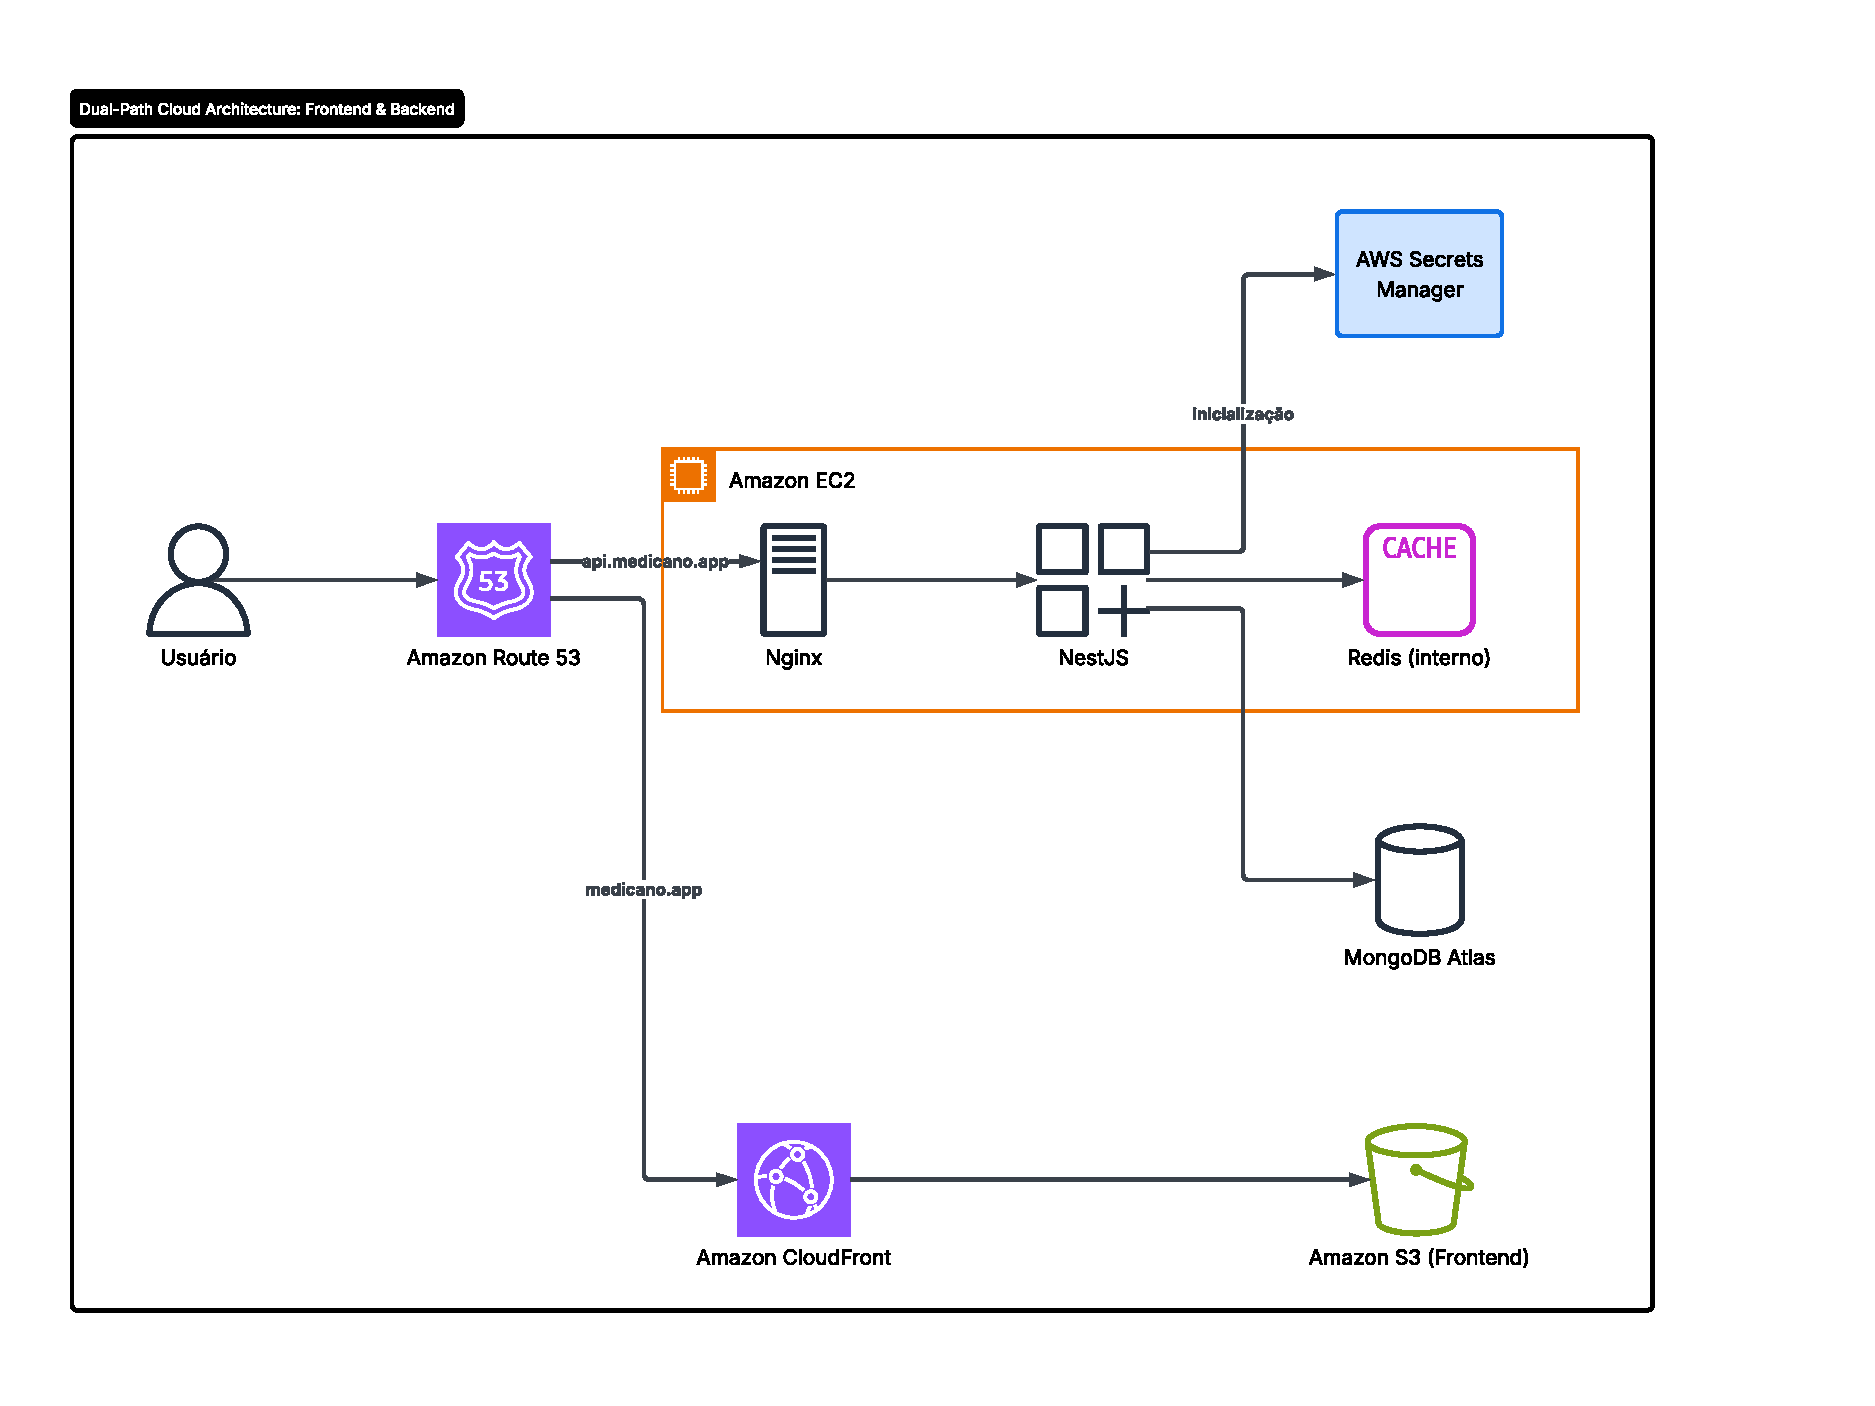
\includegraphics[width=0.95\textwidth]
    {assets/diagrams/system-architecture}
  \fonte{Elaborado pelos autores (2026)}
\end{figure}

O fluxo de uma requisição típica percorre os
seguintes componentes:

\begin{enumerate}
  \item O navegador do usuário acessa
        \texttt{medicano.app}, resolvido pelo DNS
        para o Amazon CloudFront
  \item O CloudFront entrega os arquivos estáticos
        do frontend armazenados no Amazon S3
  \item O frontend realiza chamadas à API em
        \texttt{api.medicano.app}, roteadas pelo
        DNS para a instância EC2
  \item O Nginx recebe a requisição na porta 443,
        realiza a terminação SSL e encaminha para
        o NestJS na porta 3000
  \item O NestJS processa a requisição, consultando
        o MongoDB Atlas ou o Redis conforme
        necessário
  \item A resposta percorre o caminho inverso até
        o navegador do usuário
\end{enumerate}

\section{Estrutura do Monorepo}
\label{sec:monorepo}

O código-fonte da Medicano é organizado como um
monorepo gerenciado por npm workspaces, com a
seguinte estrutura de diretórios:

\begin{figure}[H]
  \centering
  \caption{Estrutura de diretórios do monorepo}
  \label{fig:monorepo-structure}
\begin{verbatim}
medicano/
|-- apps/
|   |-- web/              frontend React + Vite
|   |-- api/              backend NestJS
|-- packages/
|   |-- types/            tipos TypeScript compartilhados
|-- docker-compose.yml    ambiente de desenvolvimento
|-- .eslintrc.js          configuração de linting
|-- .prettierrc           configuração de formatação
|-- tsconfig.base.json    configuração TypeScript base
|-- package.json          npm workspaces
\end{verbatim}
  \fonte{Elaborado pelos autores (2026)}
\end{figure}

A pasta \texttt{apps/} contém as duas aplicações
principais. A pasta \texttt{packages/types} contém
as definições de tipos TypeScript compartilhadas
entre o frontend e o backend — como enumerações de
status de agendamento, roles de usuário e interfaces
de resposta da API — evitando duplicação de
definições entre as duas camadas.

O npm workspaces permite que ambos os apps
referenciem o pacote de tipos compartilhado como
\texttt{@medicano/types}, sem necessidade de
publicação em registro externo. Um único
\texttt{npm install} na raiz instala as dependências
de todos os workspaces.

\section{Backend}
\label{sec:backend}

\subsection{Organização Modular}
\label{subsec:backend-modules}

O backend é implementado com NestJS, adotando
arquitetura modular em que cada domínio da aplicação
é encapsulado em um módulo independente com seus
próprios controllers, services e DTOs
\cite{nestjs2024}. A estrutura de módulos reflete
diretamente os domínios identificados na
especificação do sistema:

\begin{figure}[H]
  \centering
  \caption{Estrutura de módulos do backend}
  \label{fig:backend-modules}
\begin{verbatim}
apps/api/src/
|-- auth/               autenticação e autorização
|   |-- strategies/     estratégias JWT e local
|   |-- guards/         guards de rotas protegidas
|-- users/              gestão de usuários
|-- clinics/            gestão de clínicas
|-- professionals/      gestão de autônomos
|-- appointments/       agendamentos
|-- chat/               chatbot de triagem
|-- subscriptions/      planos de assinatura
|-- config/             configuração e secrets
|-- app.module.ts       módulo raiz
\end{verbatim}
  \fonte{Elaborado pelos autores (2026)}
\end{figure}

\subsection{Autenticação}
\label{subsec:auth}

O sistema de autenticação adota fluxos distintos
conforme o perfil do usuário, implementados como
estratégias separadas no módulo de autenticação:

\begin{itemize}
  \item \textbf{Paciente, clínica e autônomo:}
        autenticam por e-mail e senha. A estratégia
        valida o e-mail, verifica o hash Bcrypt da
        senha e emite um token JWT armazenado no
        Redis com TTL de 7 dias
  \item \textbf{Funcionário (atendente):}
        autentica por nome de usuário e senha dentro
        do escopo da clínica vinculada. A estratégia
        valida a combinação de \texttt{username} +
        \texttt{clinicId} para garantir unicidade
        por escopo
\end{itemize}

O guard de autenticação JWT verifica,
a cada requisição protegida, tanto a assinatura
criptográfica do token quanto sua presença no Redis,
permitindo revogação imediata no logout
\cite{rfc7519}.

\subsection{Validação de Dados}
\label{subsec:backend-validation}

Toda entrada de dados é validada por meio de DTOs
decorados com o pacote \texttt{class-validator}.
O pipe de validação global do NestJS rejeita
automaticamente requisições com dados fora do
contrato definido, retornando HTTP 400 antes de
qualquer processamento pela camada de serviço
\cite{nestjs2024}.

\subsection{Documentação da API}
\label{subsec:swagger}

A API é documentada automaticamente pelo Swagger,
integrado ao NestJS por meio do pacote
\texttt{@nestjs/swagger}. A documentação é acessível
em \texttt{api.medicano.app/api/docs} em ambiente
de desenvolvimento e está descrita de forma completa
no Apêndice~\ref{appendix:api-spec}.

\section{Frontend}
\label{sec:frontend}

O frontend é implementado com React e TypeScript,
utilizando o Vite como ferramenta de build. A
aplicação segue o padrão de Single Page Application
(SPA), com roteamento gerenciado pelo React Router
\cite{reactdev2024}.

\subsection{Organização de Pastas}
\label{subsec:frontend-structure}

\begin{figure}[H]
  \centering
  \caption{Estrutura de diretórios do frontend}
  \label{fig:frontend-structure}
\begin{verbatim}
apps/web/src/
|-- pages/              telas da aplicação
|-- components/         componentes reutilizáveis
|-- services/           chamadas à API (Axios)
|-- hooks/              hooks customizados
|-- contexts/           contextos React (auth, etc.)
|-- types/              tipos locais do frontend
|-- main.tsx            ponto de entrada
\end{verbatim}
  \fonte{Elaborado pelos autores (2026)}
\end{figure}

\subsection{Comunicação com a API}
\label{subsec:api-communication}

A camada de serviços encapsula todas as chamadas
HTTP ao backend, utilizando o Axios como cliente
HTTP. O token JWT é armazenado em memória durante
a sessão e injetado automaticamente nos cabeçalhos
de autorização por meio de um interceptor global
do Axios.

\subsection{Chatbot de Triagem}
\label{subsec:chat-frontend}

A interface do chatbot de triagem utiliza o Vercel
AI SDK no frontend para receber as respostas do
modelo em modo streaming, exibindo o texto
progressivamente enquanto ainda é gerado pelo
modelo \cite{vercelaisdk2024}. Isso proporciona
uma experiência de conversa mais fluida e natural
para o usuário.

\section{Banco de Dados}
\label{sec:database}

\subsection{MongoDB Atlas}
\label{subsec:mongodb-atlas}

O banco de dados é hospedado no MongoDB Atlas,
serviço gerenciado de banco de dados em nuvem que
oferece alta disponibilidade, backups automáticos
e monitoramento integrado \cite{sadalage2012}.
A conexão é realizada por string de conexão
armazenada no AWS Secrets Manager, nunca exposta
no código ou em variáveis de ambiente versionadas.

Os três ambientes do projeto — desenvolvimento,
\textit{staging} e produção — compartilham o mesmo
cluster Atlas M0, utilizando databases distintos
para garantir isolamento completo de dados:
\texttt{medicano\_development},
\texttt{medicano\_staging} e
\texttt{medicano\_production}. Essa estratégia
elimina a necessidade de múltiplos clusters e
mantém o comportamento do driver idêntico entre
os ambientes, reduzindo divergências de
configuração.

Para testes de integração, o MongoDB é executado
localmente em contêiner Docker \cite{docker2024},
garantindo isolamento total e reprodutibilidade
sem risco de interferência nos dados dos ambientes
remotos.

\subsection{Redis}
\label{subsec:redis-arch}

O Redis é executado na mesma instância EC2 do
backend, acessível exclusivamente por conexão
local (\texttt{localhost:6379}), sem exposição
à internet. É utilizado para armazenamento de
tokens JWT ativos com TTL automático, garantindo
revogação de sessões no logout \cite{redis2024}.

Em ambiente de desenvolvimento, o Redis também
é executado em contêiner Docker, orquestrado
pelo mesmo arquivo \texttt{docker-compose.yml}
do MongoDB.

\section{Infraestrutura}
\label{sec:infrastructure}

\subsection{Visão Geral da Infraestrutura AWS}
\label{subsec:aws-overview}

A infraestrutura de produção da Medicano é
hospedada integralmente na Amazon Web Services.
A Tabela~\ref{tab:aws-services} descreve os
serviços utilizados e suas responsabilidades.

\begin{table}[H]
  \centering
  \caption{Serviços AWS utilizados}
  \label{tab:aws-services}
  \begin{tabular}{p{3.5cm}p{7.5cm}}
    \toprule
    \textbf{Serviço} &
    \textbf{Responsabilidade} \\
    \midrule
    Amazon S3
      & Hospedagem dos arquivos estáticos do
        frontend (HTML, CSS, JavaScript) \\
    Amazon CloudFront
      & Distribuição do frontend via CDN global,
        com cache e HTTPS para \texttt{medicano.app} \\
    Amazon EC2
      & Servidor de aplicação do backend NestJS,
        com Nginx como proxy reverso \\
    Amazon Route 53
      & Gerenciamento de DNS para os domínios
        \texttt{medicano.app} e
        \texttt{api.medicano.app} \\
    AWS Secrets Manager
      & Armazenamento seguro de credenciais:
        string de conexão do MongoDB Atlas,
        segredo JWT e chaves de API dos
        modelos de linguagem \\
    AWS IAM
      & Controle de acesso entre serviços AWS,
        seguindo o princípio do menor privilégio \\
    \bottomrule
  \end{tabular}
  \fonte{Elaborado pelos autores (2026)}
\end{table}

\subsection{Configuração do EC2 e Nginx}
\label{subsec:ec2-nginx}

A instância EC2 executa o Ubuntu Server como
sistema operacional. O Nginx é configurado como
proxy reverso, recebendo requisições HTTPS na
porta 443 e encaminhando para o NestJS na porta
3000. Os certificados SSL são emitidos e renovados
automaticamente pelo Let's Encrypt por meio do
Certbot \cite{reese2008}.

A configuração de DNS é realizada pelo Amazon
Route 53, com dois registros principais:

\begin{itemize}
  \item \texttt{medicano.app} --- aponta para a
        distribuição CloudFront, servindo o
        frontend React
  \item \texttt{api.medicano.app} --- aponta para
        o IP elástico da instância EC2, servindo
        a API NestJS
\end{itemize}

\subsection{Segurança e Credenciais}
\label{subsec:security}

Todas as credenciais sensíveis são armazenadas no
AWS Secrets Manager e recuperadas pela aplicação
em tempo de execução. Nenhuma credencial é
armazenada em variáveis de ambiente versionadas,
arquivos \texttt{.env} ou no código-fonte
\cite{awssm}. O acesso ao Secrets Manager é
concedido à instância EC2 por meio de uma IAM
Role com política de leitura restrita aos secrets
do projeto, sem chaves de acesso explícitas.

\subsection{Ambientes}
\label{subsec:environments}

O projeto opera em três ambientes distintos,
diferenciados pelo prefixo dos secrets no
AWS Secrets Manager e pelo database utilizado
no cluster Atlas:

\begin{table}[H]
  \centering
  \caption{Ambientes do sistema}
  \label{tab:environments}
  \begin{tabular}{p{2.5cm}p{3.5cm}p{5cm}}
    \toprule
    \textbf{Ambiente} &
    \textbf{Prefixo dos secrets} &
    \textbf{Database no Atlas} \\
    \midrule
    Desenvolvimento
      & \texttt{medicano/development/}
      & \texttt{medicano\_development} \\
    \textit{Staging}
      & \texttt{medicano/staging/}
      & \texttt{medicano\_staging} \\
    Produção
      & \texttt{medicano/production/}
      & \texttt{medicano\_production} \\
    \bottomrule
  \end{tabular}
  \fonte{Elaborado pelos autores (2026)}
\end{table}

A variável de ambiente \texttt{NODE\_ENV} é a
única definida localmente nas máquinas de
desenvolvimento, sem conter informações sensíveis.
Com base em seu valor, o serviço de configuração
do NestJS determina qual prefixo de secret utilizar
na inicialização da aplicação.

O ambiente de \textit{staging} replica a
configuração de produção e serve para validação
de funcionalidades antes da publicação. Ele é
executado na mesma instância EC2 da produção,
em processo separado gerenciado pelo PM2, exposto
em porta distinta e sem tráfego de usuários reais.

\subsection{Escalabilidade Futura}
\label{subsec:scalability}

A arquitetura do MVP foi projetada para facilitar
a evolução sem necessidade de reescrita. As
principais evoluções planejadas para versões
futuras incluem:

\begin{itemize}
  \item Migração do Redis para Amazon ElastiCache,
        permitindo que múltiplas instâncias EC2
        compartilhem o mesmo estado de sessão
  \item Adoção de Amazon ECS ou EKS para
        orquestração de contêineres, habilitando
        escalabilidade horizontal automática do
        backend
  \item Extração do módulo de chatbot para um
        microserviço Python independente com
        LangChain, permitindo evolução da lógica
        de triagem sem impacto no backend principal
  \item Implementação de fila de mensagens com
        Amazon SQS para absorção de picos de
        demanda nas chamadas aos modelos de
        linguagem
\end{itemize}